% D3RA-DNA manuscript -- built on the official IEEEtran class (v1.8b, CTAN; the
% class IEEE distributes in its conference LaTeX template) following bare_conf.tex.
\documentclass[conference]{IEEEtran}
\IEEEoverridecommandlockouts
\usepackage{cite}
\usepackage{amsmath,amssymb,amsfonts}
\usepackage{graphicx}
\usepackage{textcomp}
\usepackage{url}
\usepackage{xcolor}
\usepackage{booktabs}
\usepackage{multirow}
\usepackage{array}
\usepackage{tikz}
\usetikzlibrary{arrows.meta,positioning,fit,shapes.geometric,calc}
\usepackage{amsthm}
\newtheorem{theorem}{Theorem}
\newtheorem{proposition}{Proposition}
\newtheorem{definition}{Definition}
\def\BibTeX{{\rm B\kern-.05em{\sc i\kern-.025em b}\kern-.08em
    T\kern-.1667em\lower.7ex\hbox{E}\kern-.125emX}}
\newcommand{\E}{\mathbb{E}}
\newcommand{\Prob}{\mathbb{P}}
\graphicspath{{figures/}}

\begin{document}

\title{Self-Calibrating Adaptive Sequencing for Exact Retrieval from Heterogeneous Multi-Container DNA Storage: Method and Evaluation on Real Read Streams}

\author{\IEEEauthorblockN{Sai Mouli}
\IEEEauthorblockA{\textit{\relax[Affiliation to be completed by the authors]}\\
\relax[City, Country]\\
\relax[e-mail]}
}

\maketitle

\begin{abstract}
DNA archives are expected to be split across many physical containers whose
sequencing efficiency, error profile and failure risk differ, yet retrieval is
usually planned with a fixed sequencing depth chosen for the worst case.  We
study how to read an erasure-coded file back \emph{exactly} from such a
heterogeneous, possibly failing set of containers with as few sequencing reads
as possible, when the containers' properties are unknown in advance.  We
present a self-calibrating controller that maintains a Bayesian posterior over
each container's efficiency (with an explicit failure atom), converts it into
per-strand recovery hazards through a hierarchical coverage model, allocates the
next batch of reads to the container with the largest expected progress per
cost, and stops only when every stripe holds $K$ verified fragments and the
file's SHA-256 matches.  To evaluate policies on \emph{real} reads rather than
simulated ones, we convert public sequencing runs into empirical recovery-time
matrices, which allow any policy to be replayed over hundreds of read orderings
with common random numbers.  On six real Illumina runs of one 12{,}000-strand
pool (ENA PRJEB65931) the controller needs 11--17\% fewer reads than a static
allocation tuned \emph{in hindsight} on the evaluation data (paired bootstrap
95\% CIs exclude zero) and, combined with placement, 34\% fewer than uniform
fixed-depth retrieval; on an independent 12{,}472-strand pool from a different
vendor the corresponding figures are 11\% and 63\%.  Starting from a generic
literature prior with no calibration reads, the controller matches full calibration
on the first pool and costs 4--5\% more than in-pool calibration on the second, still
10\% below the hindsight-tuned static plan.  It flags strongly degraded containers
after about one to two reads per stored strand with no false alarms on near-nominal
containers.  We also report negative results: the stripe-importance scoring rule
is no better than a simpler hazard-greedy rule; the posterior's credible intervals
are over-confident (an exploratory overdispersed likelihood largely fixes this on a
held-out pool); its predicted completion probability is under-confident and
an early-abandonment rule built on it is harmful; and our analytical surrogate is
5--18\% optimistic on one pool and 3.7$\times$ pessimistic on the other.  All
results are computational; no new synthesis or sequencing was
performed.
\end{abstract}

\begin{IEEEkeywords}
DNA data storage, adaptive sequencing, Bayesian calibration, erasure coding, coverage depth, sequential decision making, reproducibility
\end{IEEEkeywords}

%=====================================================================
\section{Introduction}
%=====================================================================
DNA has been demonstrated as an archival medium at megabyte to hundreds-of-megabyte
scale~\cite{church2012next,goldman2013towards,grass2015robust,erlich2017fountain,organick2018random}.
Retrieval requires sequencing, which samples molecules at random: some strands are read
many times, others never, and every read carries substitution, insertion and deletion
errors~\cite{heckel2019characterization,gimpel2023digital}.  Systems therefore protect each
strand with an inner code, protect groups of strands with an outer erasure code, and sequence
to a fixed depth that is expected to recover enough strands~\cite{grass2015robust,organick2018random}.
The number of reads needed for decoding---the \emph{coverage depth}---has recently become an
object of study in its own right~\cite{barlev2025cover,gruica2024combinatorial}.

Practical archives will not be a single homogeneous pool.  Capacity, random access and risk
management push towards many physical containers (vials, capsules, pools) that are written,
stored and handled separately~\cite{bornholt2016dna,organick2018random}.  Recent theory
considers erasure-coded data partitioned across containers with uniform
sampling~\cite{kong2026coverage} and expected recovery time when containers
fail~\cite{levy2026expected}.  Two operational questions remain open in this setting:
(i) containers differ---one has been amplified more often, another has aged---and these
differences are not known when retrieval starts; (ii) a fixed sequencing plan must pay for the
rare slow case on every retrieval.

\textbf{Problem.}  Given an erasure-coded file distributed over $M$ containers of unknown and
heterogeneous efficiency, some of which may have failed, sequence in batches and decide after
each batch which container to read next and when to stop, so that the file is recovered
\emph{exactly} (byte-identical, hash-verified) with high probability while minimising the
number (cost) of reads.

\textbf{Contributions.}  We are explicit about what is new and what is not; a verified prior-art
assessment is given in Section~\ref{sec:related}.
\begin{enumerate}
\item A \emph{self-calibrating retrieval controller} that couples a discrete Bayesian posterior
over container efficiency (including container failure) with a hierarchical strand-recovery
hazard model, allocates reads greedily by expected progress per cost and stops on verified
decodability (Section~\ref{sec:method}).  Stopping when decodable and checksum gating are
known practice~\cite{lopez2019dna}; the container-selection component has no direct precedent
we could find in DNA storage, but has analogues in adaptive sampling and bandits
(Section~\ref{sec:related}).
\item An evaluation methodology that turns public sequencing runs into \emph{empirical
recovery-time matrices}, so that placement and retrieval policies can be compared on real
reads with common random numbers, including a strongest-possible static baseline tuned in
hindsight (Section~\ref{sec:eval}).
\item An empirical study on two independent real pools and on controlled simulations
answering five research questions (generalisation to unfamiliar pools, calibration from
limited observations, detection of efficiency changes, cost reduction, and exact recovery
under failures), including negative results (Section~\ref{sec:results}).
\item Supporting channel results: on two independent nanopore flowcells, a strand-specific
error component persists across runs and a hierarchical beta-binomial error model predicts
consensus success 2.2$\times$ more accurately than an i.i.d.\ model (Section~\ref{sec:channel}).
\end{enumerate}
Everything reported is computational: the experiments re-use public sequencing data and
simulation; no DNA was synthesised or sequenced for this work.

%=====================================================================
\section{Background and Related Work}\label{sec:related}
%=====================================================================
\textbf{DNA storage systems and channels.}  Storage systems combine constrained encodings with
inner and outer codes~\cite{antkowiak2020low,goldman2013towards,grass2015robust,erlich2017fountain,organick2018random,press2020hedges}.
Channel studies show that coverage is over-dispersed (approximately negative binomial or
log-normal), that a few percent of strands drop out, and that errors arise mostly in synthesis
and sequencing~\cite{heckel2019characterization,chen2020quantifying,gimpel2023digital}.
Information-theoretic models treat the channel as sampling with replacement followed by
noise~\cite{shomorony2021dna,weinberger2022dna,lenz2020coding}.

\textbf{Coverage depth.}  Bar-Lev \emph{et al.} define the coverage-depth problem and show that,
for a sampler that cannot be controlled, MDS codes and uniform sampling minimise the expected
number of reads, which equals $n(H_n-H_{n-k})$ for an $[n,k]$ MDS code~\cite{barlev2025cover}.
Follow-ups study random access~\cite{gruica2024combinatorial}, real-data sampling
distributions~\cite{cao2025optimizing}, partitioning over containers~\cite{kong2026coverage}
and container failures~\cite{levy2026expected}, and the reliability of MDS-coded retrieval has been analysed~\cite{kashanna2026reliability}.  These works analyse \emph{fixed} sampling laws;
we study a \emph{controllable} sampler that learns which container to read.

\textbf{Adaptive sequencing and sequential decisions.}  Nanopore ``Read Until'' and adaptive
sampling select molecules in real time~\cite{loose2016real,payne2021readfish,weilguny2023dynamic};
DNA-storage readouts have been sequenced until sufficient coverage was
reached~\cite{lopez2019dna}.  Choosing which container to read so as to complete $K$-of-$N$
stripes resembles adaptive coupon collection with a controllable sampler, which has analogues
in bandit problems~\cite{thompson1933likelihood,bubeck2013optimal}.

\textbf{Placement across failure domains.}  Erasure-coded storage limits the number of fragments
of a stripe per failure domain~\cite{weil2006crush,cidon2013copysets,ford2010availability};
spreading can be worse than concentrating under correlated failures~\cite{nath2006subtleties},
and the optimal allocation of coded storage across unreliable nodes was characterised by Leong
\emph{et al.}~\cite{leong2012distributed}.  Our spreading rule (Section~\ref{sec:theory}) is a
special case of their analysis and is stated only as a design rule.

\textbf{Consensus and correlated errors.}  Strands are reconstructed from noisy reads by trace
reconstruction~\cite{batu2004reconstructing,srinivasavaradhan2021trellis,sabary2024reconstruction} after clustering~\cite{rashtchian2017clustering} or learned
models~\cite{barlev2025deep}; systematic, context-dependent nanopore errors are well
documented~\cite{delahaye2021sequencing,wick2019performance}.

Table~\ref{tab:literature_comparison} compares the closest works.  The gap we address is the combination of
(a) unknown, heterogeneous container efficiency that must be learned online, (b) container
failures, (c) a controllable, adaptive read allocation with a verified stopping rule, and
(d) evaluation on real read streams from more than one pool.
% literature_comparison.tex -- comparison of the closest prior work (see supplementary/literature_review.md, Sec. 13).
% Entries reflect only what each paper does (Kong et al.: abstract only). Requires \usepackage{booktabs}.
% Y = yes, N = no, P = partial, I = implicit (reads-until-decodable analysed, no operational rule), -- = not stated.
\begin{table*}[!t]
\centering
\caption{Positioning against the closest prior work. Y: yes; N: no; P: partial; I: implicit (expected reads until
decodability analysed, no operational stopping rule); --: not stated. ``Containers'' in \cite{leong2012distributed} are
storage nodes, and in \cite{bubeck2013optimal} they are sampling sources (``experts'').}
\label{tab:literature_comparison}
\footnotesize
\setlength{\tabcolsep}{4pt}
\begin{tabular}{@{}lccccccc@{}}
\toprule
Work & Multi- & Container & Heterog. & Correlated & Adaptive read & Stopping & Real-data \\
     & container & failures & containers & errors & allocation & rule & evaluation \\
\midrule
Lopez et al.\ 2019 \cite{lopez2019dna}                      & N & N & N & -- & N & P & Y \\
Gimpel et al.\ 2023 \cite{gimpel2023digital}                & N & N & P & N & N & N & Y \\
Bar-Lev et al.\ 2025 \cite{barlev2025cover}                 & N & N & N & N & N & I & N \\
Gruica et al.\ 2024 \cite{gruica2024combinatorial}          & N & N & N & N & N & I & N \\
Cao \& Chen 2025 \cite{cao2025optimizing}                   & N & N & N & N & N & I & P \\
Kas Hanna 2026 \cite{kashanna2026reliability}               & N & N & N & N & N & N & N \\
Levy et al.\ 2026 \cite{levy2026expected}                   & Y & Y & N & N & N & I & N \\
Kong et al.\ 2026 \cite{kong2026coverage}                   & Y & N & P & N & N & I & N \\
Leong et al.\ 2012 \cite{leong2012distributed}              & Y & Y & N & N & N & N & N \\
Weilguny et al.\ 2023 \cite{weilguny2023dynamic}            & N & N & -- & N & Y & -- & Y \\
Bubeck et al.\ 2013 \cite{bubeck2013optimal}                & Y & N & Y & N & Y & N & N \\
\midrule
This work                                                   & Y & Y$^{a}$ & Y & Y & Y & Y & Y$^{b}$ \\
\bottomrule
\end{tabular}

\vspace{2pt}
\parbox{\textwidth}{\scriptsize $^{a}$Failures injected on real read streams; real failure rates are not measured.
$^{b}$ENA PRJEB65931 \cite{gimpel2023prjeb65931} (same-batch aliquots), Zenodo 17473983 \cite{technion2025dnaformerreads}
and 14296588 \cite{barlev2024binned}. Gimpel et al.\ \cite{gimpel2023digital}: heterogeneity characterised across
handling conditions of one pool. Cao \& Chen \cite{cao2025optimizing}: log-normal channel fitted to their own data.
Weilguny et al.\ \cite{weilguny2023dynamic}: genomic loci, not storage containers.}
\end{table*}


%=====================================================================
\section{System Model and Problem Formulation}\label{sec:model}
%=====================================================================
Fig.~\ref{fig:arch} shows the architecture, Fig.~\ref{fig:hier} the model hierarchy and Table~\ref{tab:notation} the notation.

\begin{figure*}[t]
\centering
\resizebox{\textwidth}{!}{%
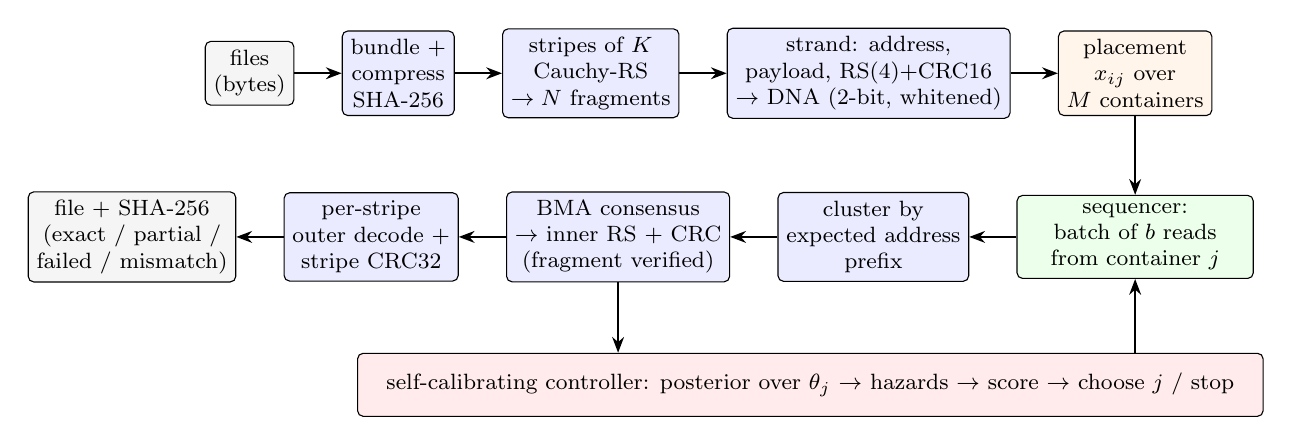
\begin{tikzpicture}[font=\footnotesize, node distance=4mm and 6mm,
  box/.style={draw, rounded corners=2pt, align=center, minimum height=8mm, inner sep=3pt, fill=#1!8},
  box/.default=blue, arr/.style={-{Stealth[length=2mm]}, thick}]
\node[box=gray] (files) {files\\(bytes)};
\node[box, right=of files] (bundle) {bundle +\\compress\\SHA-256};
\node[box, right=of bundle] (stripes) {stripes of $K$\\Cauchy-RS\\$\to N$ fragments};
\node[box, right=of stripes] (strands) {strand: address,\\payload, RS(4)+CRC16\\$\to$ DNA (2-bit, whitened)};
\node[box=orange, right=of strands] (place) {placement\\$x_{ij}$ over\\$M$ containers};
\node[box=green, below=10mm of place, minimum width=30mm] (seq) {sequencer:\\batch of $b$ reads\\from container $j$};
\node[box, left=of seq] (clus) {cluster by\\expected address\\prefix};
\node[box, left=of clus] (cons) {BMA consensus\\$\to$ inner RS + CRC\\(fragment verified)};
\node[box, left=of cons] (outer) {per-stripe\\outer decode +\\stripe CRC32};
\node[box=gray, left=of outer] (out) {file + SHA-256\\(exact / partial /\\failed / mismatch)};
\node[box=red, below=9mm of clus, minimum width=115mm, xshift=-8mm] (ctl) {self-calibrating controller: posterior over $\theta_j$ $\to$ hazards $\to$ score $\to$ choose $j$ / stop};
\draw[arr] (files)--(bundle); \draw[arr] (bundle)--(stripes); \draw[arr] (stripes)--(strands); \draw[arr] (strands)--(place);
\draw[arr] (place)--(seq); \draw[arr] (seq)--(clus); \draw[arr] (clus)--(cons); \draw[arr] (cons)--(outer); \draw[arr] (outer)--(out);
\draw[arr] (cons.south) -- (cons.south |- ctl.north); \draw[arr] (seq.south |- ctl.north) -- (seq.south);
\end{tikzpicture}}
\caption{D3RA-DNA architecture (conceptual diagram).  Storage path (top), retrieval path
(middle) and the closed control loop (bottom): verified fragment recoveries update the
container posterior, which chooses the next container to sequence and decides when to stop.}
\label{fig:arch}
\end{figure*}


\begin{figure}[t]
\centering
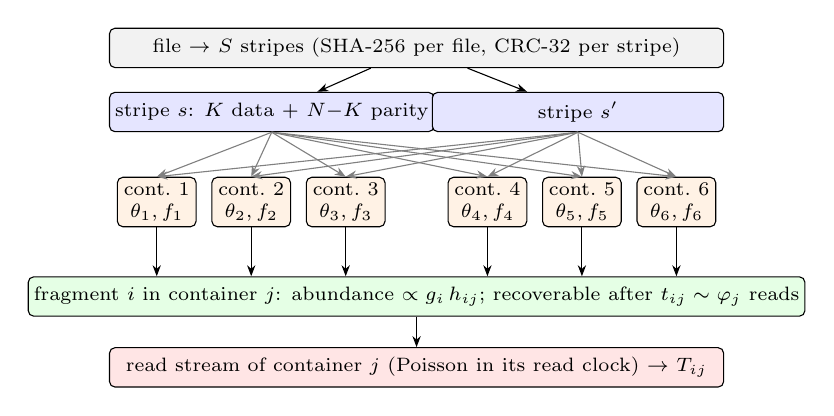
\begin{tikzpicture}[font=\scriptsize, >={Stealth[length=1.4mm]},
  lv/.style={draw, rounded corners=2pt, fill=#1!10, minimum height=5mm, inner sep=2pt, align=center}]
\node[lv=gray, minimum width=78mm] (file) {file $\to$ $S$ stripes (SHA-256 per file, CRC-32 per stripe)};
\node[lv=blue, below=3mm of file.south west, anchor=north west, minimum width=37mm] (s1) {stripe $s$: $K$ data + $N{-}K$ parity};
\node[lv=blue, below=3mm of file.south east, anchor=north east, minimum width=37mm] (s2) {stripe $s'$};
\foreach \k/\x in {1/-33,2/-21,3/-9,4/9,5/21,6/33} \node[lv=orange, minimum width=10mm] (c\k) at ($(file.south)+(\x mm,-17mm)$) {cont.\ \k\\$\theta_\k, f_\k$};
\node[lv=green, minimum width=78mm] (frag) at ($(file.south)+(0,-29mm)$) {fragment $i$ in container $j$: abundance $\propto g_i\,h_{ij}$; recoverable after $t_{ij}\sim\varphi_j$ reads};
\node[lv=red, minimum width=78mm] (rd) at ($(file.south)+(0,-38mm)$) {read stream of container $j$ (Poisson in its read clock) $\to$ $T_{ij}$};
\draw[->] (file) -- (s1); \draw[->] (file) -- (s2);
\foreach \k in {1,...,6} {\draw[->,gray] (s1.south) -- (c\k.north); \draw[->,gray] (s2.south) -- (c\k.north); \draw[->] (c\k.south) -- (c\k.south |- frag.north);}
\draw[->] (frag) -- (rd);
\end{tikzpicture}
\caption{Hierarchy of the model (conceptual diagram): stripes are spread over containers by
the placement $x_{ij}$ (grey arrows); each container has an unknown efficiency $\theta_j$ and failure
probability $f_j$; a strand's abundance has a shared ($g_i$) and a container-specific
($h_{ij}$) component.}
\label{fig:hier}
\end{figure}
\begin{table}[!t]
\centering
\caption{Notation (code objects in package \texttt{d3ra}).}
\label{tab:notation}
\scriptsize
\setlength{\tabcolsep}{3pt}
\begin{tabular}{@{}>{\raggedright\arraybackslash}p{13mm}>{\raggedright\arraybackslash}p{44mm}>{\raggedright\arraybackslash}p{26mm}@{}}
\toprule
Symbol & Meaning & Code \\
\midrule
$K,N,S,P$ & data / total fragments per stripe, stripes, payload bytes & \texttt{erasure\_codes} \\
$M$, $j$ & number of containers, container index & \texttt{Layout} \\
$n_j$ & fragments stored in container $j$ & \texttt{Layout} \\
$b$ & batch size (reads per decision) & \texttt{AdaptiveConfig} \\
$R_j$, $U_j$ & reads taken from $j$, verified fragments from $j$ & \texttt{StreamRetriever} \\
$\theta_j$, $\Theta$, $s$ & efficiency multiplier, its grid, prior log-sd & \texttt{AdaptiveConfig} \\
$f_j$ & prior probability that container $j$ failed & \texttt{ChannelParams} \\
$\bar\pi_j$ & prior per-fragment read share of container $j$ & \texttt{Adaptive}\allowbreak\texttt{Controller} \\
$k$, $d$, $\varphi(t)$ & NB shape, dropout, consensus-success curve & \texttt{ChannelParams} \\
$Q(\mu)$ & P(fragment decodable) at mean coverage $\mu$ & \texttt{\_QTable} \\
$\rho_U$ & beta-binomial ICC of recoveries in the likelihood & \texttt{overdispersion} \\
$h_{ij}$ & hazard of recovery within the next batch & \texttt{scores} \\
$q$ & posterior quantile for UCB ($q$) and tail-aware ($1{-}q$) & \texttt{quantile} \\
$\nu_s$ & remaining need of stripe $s$ ($K$ minus verified) & \texttt{scores} \\
$w_j$, $e_j$, $\alpha$ & static proportions, hindsight per-read recovery rate, exponent & \texttt{static\_family} \\
$\theta^\ast_j$ & calibration target (best-fitting multiplier) & \texttt{\_theta\_star} \\
q99 & 0.99-quantile of reads per retrieval & \texttt{dt\_analysis} \\
\bottomrule
\end{tabular}
\end{table}


\subsection{Storage}
A file (or bundle of files, optionally compressed) is split into $S$ stripes of $K$ data
fragments of $P{=}32$ bytes.  A systematic Cauchy Reed--Solomon code~\cite{reed1960polynomial} over $\mathrm{GF}(2^8)$
extends each stripe to $N$ fragments; any $K$ suffice (MDS).  Each fragment becomes a strand
carrying a compact address, an address check byte, the payload and an inner Reed--Solomon code
with four parity bytes plus a 16-bit CRC, mapped to DNA by a whitened 2-bit code (168--172\,nt).
Logical metadata (code parameters, per-stripe CRC-32, SHA-256 of the blob and of every file)
is kept in a manifest outside the DNA.  Placement $x_{ij}\in\{0,1\}$ assigns fragment $i$ to
container $j$.  Our default geometry is $K{=}32$, $N{=}48$.

\subsection{Sequencing and recovery (hierarchical model)}
Reads from container $j$ are a Poisson process in that container's \emph{read clock}.  A read
originates from stored fragment $i$ with probability
\begin{equation}
\pi_{ij}=y_j\,\frac{x_{ij}\,g_i\,h_{ij}}{\sum_{i'}x_{i'j}\,g_{i'}\,h_{i'j}},\qquad
\begin{aligned}g_i&\sim\mathrm{LogN}(-\tfrac{\sigma_g^2}{2},\sigma_g^2),\\ h_{ij}&\sim\Gamma(k_j,1/k_j),\end{aligned}
\label{eq:abundance}
\end{equation}
where $y_j$ is the usable yield, $g_i$ a strand effect shared by all containers holding $i$
(synthesis-batch bias) and $h_{ij}$ a container-specific effect.  A fragment's cluster in
container $j$ becomes decodable once it holds $t_{ij}$ reads, with
$\Prob(t_{ij}\le n)=\varphi_j(n)$, the consensus-success curve.  Molecules are absent with
probability $d_j$ (dropout) and a container fails entirely with probability $f_j$.  Hence the
number of container-$j$ reads at which pair $(i,j)$ becomes recoverable is
\begin{equation}
T_{ij}=\Gamma(t_{ij},1)/\pi_{ij}\quad(\infty\text{ if absent or failed}).
\label{eq:T}
\end{equation}
Given cumulative reads $R=(R_j)$, fragment $i$ is recovered iff $\min_j(T_{ij}-R_j)\le0$, and
the file is decodable iff every stripe has $\ge K$ recovered fragments.  Integrating
\eqref{eq:abundance} over $h_{ij}$ gives negative-binomial read counts, and over $g_i$ (by
Gauss--Hermite quadrature) the decodability of a pair after $R_j$ reads,
\begin{equation}
Q_j(\mu)=(1-d_j)\,\E_g\Big[\sum_{n\ge0}\mathrm{NB}(n;k_j,g\mu)\,\varphi_j(n)\Big]
\label{eq:Q}
\end{equation}
evaluated at $\mu=R_j\bar\pi_{ij}$ with $\bar\pi_{ij}=y_j x_{ij}/\sum_{i'}x_{i'j}$ (synthesis dropout, shared by all copies of a fragment, multiplies $Q_j$ in the code).

\subsection{Objective}
A retrieval policy $\pi$ chooses, after each batch, a container and whether to stop.  With
read costs $c_j$ and a failure budget $\varepsilon$ we seek
\begin{equation}
\begin{aligned}&\min_{\pi}\ \E\big[\min(C_\pi, B_\varepsilon)\big]\\ &\text{s.t.}\ \ \Prob\big(\text{exact recovery within }B_\varepsilon\big)\ge1-\varepsilon,\end{aligned}
\label{eq:objective}
\end{equation}
where $C_\pi=\sum_j c_jR_j$ at stopping and the cap $B_\varepsilon$ is the
$(1{-}\varepsilon)$-quantile of $C_\pi$.  For a static plan, which commits read fractions
$w$ and a budget in advance, the expected spend equals its budget.  We report the
\emph{expected spend at 0.99} ($\varepsilon{=}0.01$) throughout.

%=====================================================================
\section{Proposed Method}\label{sec:method}
%=====================================================================
\begin{figure}[t]
\centering
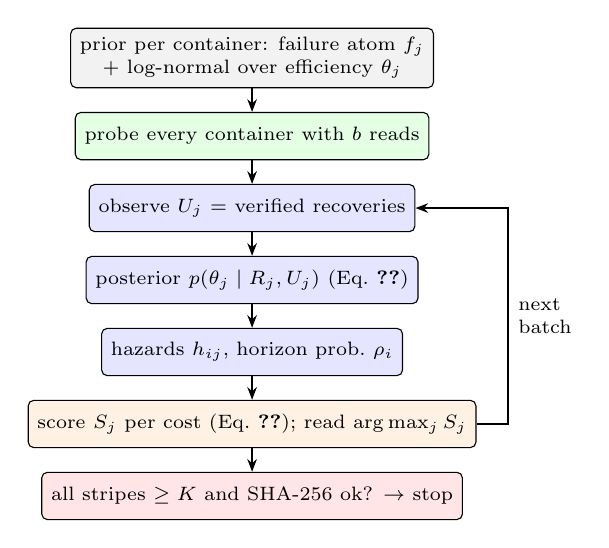
\begin{tikzpicture}[font=\scriptsize, node distance=3mm,
  b/.style={draw, rounded corners=2pt, align=center, fill=#1!10, minimum width=34mm, minimum height=6mm},
  b/.default=blue, arr/.style={-{Stealth[length=1.6mm]}, thick}]
\node[b=gray] (prior) {prior per container: failure atom $f_j$\\ + log-normal over efficiency $\theta_j$};
\node[b=green, below=of prior] (probe) {probe every container with $b$ reads};
\node[b, below=of probe] (obs) {observe $U_j$ = verified recoveries};
\node[b, below=of obs] (post) {posterior $p(\theta_j\mid R_j,U_j)$ (Eq.~\ref{eq:posterior})};
\node[b, below=of post] (haz) {hazards $h_{ij}$, horizon prob.\ $\rho_i$};
\node[b=orange, below=of haz] (score) {score $S_j$ per cost (Eq.~\ref{eq:score}); read $\arg\max_j S_j$};
\node[b=red, below=of score] (stop) {all stripes $\ge K$ and SHA-256 ok? $\to$ stop};
\foreach \a/\c in {prior/probe,probe/obs,obs/post,post/haz,haz/score,score/stop} \draw[arr] (\a)--(\c);
\draw[arr] (score.east) -- ++(4mm,0) |- (obs.east) node[pos=0.25,right,align=left]{next\\batch};
\end{tikzpicture}
\caption{Self-calibration and allocation loop of the controller (conceptual diagram).}
\label{fig:loop}
\end{figure}

\subsection{Online Bayesian calibration}
Each container's unknown deviation from its prior model is summarised by a single efficiency
multiplier $\theta_j$ that scales its read rate; $\theta_j=0$ represents a failed container.
The support is $\Theta=\{0\}\cup\{\theta^{(1)},\dots,\theta^{(25)}\}$ with log-spaced
$\theta^{(\ell)}\in[0.01,5]$ and the prior
$p_0(\theta{=}0)=f_j$, $p_0(\theta^{(\ell)})\propto(1-f_j)\exp(-\tfrac12(\ln\theta^{(\ell)}/s)^2)$,
where $s$ (\texttt{prior\_sd}) encodes how much the container may deviate from the prior model.
After $R_j$ reads with $U_j$ verified recoveries among the $n_j$ stored fragments,
\begin{equation}
p(\theta\mid R_j,U_j)\propto p_0(\theta)\,\mathrm{Bin}\big(U_j;\,n_j,\,Q_j(\theta R_j\bar\pi_j)\big),
\label{eq:posterior}
\end{equation}
with $p(\theta{=}0)=0$ as soon as $U_j>0$.  This single object absorbs mis-estimated yield,
abundance, error rate and container failure.  We keep the support down to $\theta{=}0.01$: with
a floor of $0.2$, a heavily degraded container whose probe returned nothing was classified as
failed and abandoned in an earlier version of the controller.

\subsection{Recovery hazards and allocation}
For an unrecovered pair, the posterior-plug-in probability of recovery within $\Delta$ more
reads (the hazard) is
\begin{equation}
h_{ij}(\Delta)=\frac{Q_j(\hat\theta_j(R_j{+}\Delta)\bar\pi_{ij})-Q_j(\hat\theta_jR_j\bar\pi_{ij})}{1-Q_j(\hat\theta_jR_j\bar\pi_{ij})},
\label{eq:hazard}
\end{equation}
with $\hat\theta_j$ the posterior mean.  Conditioning on ``not yet recovered'' automatically
lowers the presence probability of long-missing molecules.  Let $\nu_s=\max(K-U^{(s)},0)$ be
the remaining need of stripe $s$ and $\rho_i$ the probability that fragment $i$ is recovered
within a look-ahead horizon $H$ ($6$ batches per container).  With
$\mu_s=\sum_{i\in s}\rho_i$, $\sigma_s^2=\sum_{i\in s}\rho_i(1-\rho_i)+\tfrac14$ and
$z_s=(\mu_s-\nu_s+\tfrac12)/\sigma_s$, the stripe weight is
$W_s=\phi(z_s)/(\sigma_s\Phi(z_s))$, the normal approximation of
$\partial\log\Prob(\textstyle\sum_{i\in s}X_i\ge\nu_s)/\partial\rho_i$ (a Birnbaum-type component importance).  The controller reads the container maximising
\begin{equation}
S_j=\frac{\sum_{(i,j)\ \text{open}}W_{s(i)}\,h_{ij}(b)\,\big(1-\rho_i+h_{ij}(b)\big)}{c_jb+c^{\mathrm{setup}}_j}.
\label{eq:score}
\end{equation}
The simpler \emph{coverage-greedy} rule drops $W_s$ and $\rho_i$:
$S_j=\sum h_{ij}(b)/(c_jb+c_j^{\mathrm{setup}})$ over fragments of unfinished stripes.

\subsection{Verified stopping and posterior predictive completion}
The controller stops with ``exact'' only when (i) every stripe holds $K$ fragments that each
passed inner RS decoding, CRC-16 and the address check, (ii) every stripe matches its
per-stripe CRC-32, and (iii) the file matches its SHA-256.  If (ii) fails, the controller
requests one more fragment for that stripe and localises the faulty fragment by leave-one-out
decoding.  A wrong file is therefore output only on a SHA-256 collision; the risk of stopping
is entirely moved into cost.  The controller also estimates the posterior predictive
probability of completing within the remaining budget,
\begin{equation}
\hat P_{\mathrm{complete}}=\prod_s\Phi\!\left(\frac{\sum_{i\in s}\rho^{\mathrm{rem}}_i-\nu_s+\frac12}{\sqrt{\sum_{i\in s}\rho^{\mathrm{rem}}_i(1-\rho^{\mathrm{rem}}_i)}}\right),
\label{eq:pcomplete}
\end{equation}
with $\rho^{\mathrm{rem}}_i$ computed from \eqref{eq:hazard} with the remaining budget spread
over containers.  We evaluate its calibration in Section~\ref{sec:results}.

\subsection{Correlated errors}\label{sec:channel}
Consensus success $\varphi_j(n)$ depends on whether errors repeat across reads of a strand.
We model a persistent per-position error propensity
\begin{equation}
p_{sp}\sim\mathrm{Beta}\!\Big(\mu_{c(s,p)}\tfrac{1-\rho}{\rho},\,(1-\mu_{c(s,p)})\tfrac{1-\rho}{\rho}\Big),
\label{eq:betabin}
\end{equation}
where $\mu_c$ is the error rate of the local context $c$ (5-mer and homopolymer run) and
$\rho$ the intra-class correlation of errors across reads; each read errs at $p$ with
probability $p_{sp}$, so the error count at $(s,p)$ over $n$ reads is beta-binomial.  The
method-of-moments estimate follows from
$\E[(\bar x_{sp}-\mu)^2]=\mu(1-\mu)/n+\rho\,\mu(1-\mu)(1-1/n)$.  In the experiments the
controller uses $\varphi_j$ calibrated from real reads; the beta-binomial model is evaluated
as a predictor of $\varphi$ (Section~\ref{sec:res-channel}) and is not yet coupled into the
controller.

\subsection{Placement rule}\label{sec:theory}
For $D$ failure domains failing independently with probability $q$, an even split of an
$(N,K)$ MDS stripe tolerates $t=\lfloor D\rho_{\mathrm{par}}\rfloor$ domain losses, where
$\rho_{\mathrm{par}}=(N-K)/N$.  If $\rho_{\mathrm{par}}<1/D$, even spreading is worse than
concentrating in one domain for every $q\in(0,1)$; if $t\ge1$, spreading is better iff
$q<q^\star(D,t)$, the unique root of $\Prob(\mathrm{Bin}(D,q)\ge t{+}1)=q$ (e.g.\ $q^\star=0.232$
for $D{=}4,t{=}1$).  This follows from the allocation analysis of~\cite{leong2012distributed};
a proof, a dropout-margin correction and a heterogeneous extension are given in the
supplementary material; the sign prediction was correct in all 8{,}148 covered cases of an independent numerical reproduction.  We use it only to choose
placements.

%=====================================================================
\section{Implementation}
%=====================================================================
D3RA-DNA is a Python package (NumPy, SciPy, \texttt{reedsolo}, \texttt{edlib}) with 201 unit
and integration tests.  The full path store $\rightarrow$ FASTQ $\rightarrow$ retrieve runs on
disk: \texttt{d3ra store} writes a manifest, the placement and per-container synthesis FASTA
files; \texttt{d3ra simulate} writes one FASTQ per container (optionally with real error
scripts transplanted from public reads); \texttt{d3ra retrieve} streams the FASTQ files in
batches, clusters reads against the expected address prefixes (computable from the manifest),
runs two-sided bitwise-majority-alignment consensus~\cite{batu2004reconstructing} (forward-only
for raw reads with untrimmed 3$'$ tails), inner decoding, outer decoding with per-stripe
verification, and writes SHA-256-verified files.  The controller is vectorised over
Monte-Carlo trials.  Code, configuration, seeds and result files are listed in
Section~\ref{sec:repro}.

%=====================================================================
\section{Evaluation Methodology}\label{sec:eval}
%=====================================================================
\subsection{Empirical recovery-time matrices from real reads}
Sequencing reads are independent draws from a sample.  A container that holds a subset of
strands therefore produces exactly the sample's read stream restricted to that subset (plus a
proportional share of unmappable reads).  For a real run $j$ and strand $i$ we (1) map reads to
designed strands (k-mer voting, edit-distance verification; 99.5\% mapped), (2) estimate a
strand-specific empirical consensus curve $\hat\varphi_{ij}(n)$ by repeatedly taking $n$ of the
strand's real reads, computing the consensus and checking it against the design, and (3) for
each trial draw a random permutation of the run's evaluation reads and set $T_{ij}$ to the
stream position of the $t_{ij}$-th read of strand $i$, $t_{ij}\sim\hat\varphi_{ij}$.  The
resulting matrix replaces \eqref{eq:T}; any static or adaptive policy is then replayed on the
same matrices (common random numbers).  For a static plan with read fractions $w$ the minimal
budget of a trial is closed-form,
$B^\star(w)=\max_s\operatorname{ord}_{K}\{\min_jT_{ij}/w_j: i\in s\}$.
Beliefs used by the controller are estimated from a disjoint \emph{calibration} split of reads
(the first 300k reads of each run; evaluation uses the next 900k), except where stated.

\begin{figure}[t]
\centering
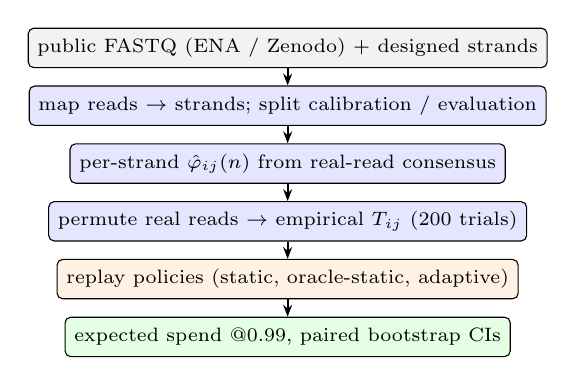
\begin{tikzpicture}[font=\scriptsize, node distance=2.2mm,
 s/.style={draw, rounded corners=2pt, align=center, fill=#1!10, minimum width=36mm, minimum height=5mm}, s/.default=blue,
 arr/.style={-{Stealth[length=1.5mm]}, thick}]
\node[s=gray] (a) {public FASTQ (ENA / Zenodo) + designed strands};
\node[s, below=of a] (b) {map reads $\to$ strands; split calibration / evaluation};
\node[s, below=of b] (c) {per-strand $\hat\varphi_{ij}(n)$ from real-read consensus};
\node[s, below=of c] (d) {permute real reads $\to$ empirical $T_{ij}$ (200 trials)};
\node[s=orange, below=of d] (e) {replay policies (static, oracle-static, adaptive)};
\node[s=green, below=of e] (f) {expected spend @0.99, paired bootstrap CIs};
\foreach \x/\y in {a/b,b/c,c/d,d/e,e/f} \draw[arr] (\x)--(\y);
\end{tikzpicture}
\caption{Experimental pipeline for real-data evaluation (conceptual diagram).}
\label{fig:pipeline}
\end{figure}

\subsection{Data}
\textbf{Twist pool:} six Illumina iSeq runs (ENA PRJEB65931~\cite{gimpel2023digital,gimpel2023prjeb65931}) of one
12{,}000-strand (108\,nt) pool after aging for 0/2/7 days or 15/60/90 PCR cycles; designs from
the DT4DDS release.  \textbf{Genscript pool:} an independent pool from another vendor
(12{,}472 strands of 102\,nt), six runs (aging 0\,d replicates A/B, 2\,d, 7\,d; PCR 15/30
cycles).  \textbf{Nanopore:} DNAformer binned reads of 55{,}000 strands on two separate
flowcells~\cite{barlev2025deep,technion2025dnaformerreads} and the clustered reads of~\cite{srinivasavaradhan2021trellis,barlev2024binned}.
We place 12{,}000 strands in 250 stripes of $(K,N)=(32,48)$; each run acts as one container.

\subsection{Baselines and metrics}
\emph{Fixed depth}: uniform read fractions with the budget equal to the 0.99-quantile of its
own per-trial requirement on the evaluation data (optimistic: the budget is known in
hindsight).  \emph{Oracle-tuned static}: read fractions optimised by Nelder--Mead directly on
the evaluation matrices---no deployable static plan can do better.  \emph{Adaptive stop,
round-robin}: our stopping rule with uniform allocation.  \emph{Adaptive (proposed)}: pivotal
and coverage-greedy scores.  The primary metric is expected spend at 0.99
(\eqref{eq:objective}); differences are reported with paired bootstrap 95\% CIs over the same
read permutations (2{,}000 resamples~\cite{efron1993introduction}; effect sizes as Cliff's $\delta$~\cite{cliff1993dominance}).  Experimental settings are summarised in
Table~\ref{tab:config}.
\begin{table}[!t]
\centering
\caption{Experimental configuration (all values as in the committed scripts).}
\label{tab:config}
\scriptsize
\begin{tabular}{@{}p{30mm}p{48mm}@{}}
\toprule
Item & Setting \\
\midrule
Outer code & Cauchy RS over GF($2^8$), $(K,N)=(32,48)$ \\
Inner code & RS, 4 parity bytes + CRC-16 + address check \\
Real-data layout & 250 stripes $\times$ 48 = 12{,}000 strands \\
Containers & 6 runs per pool, each one container \\
Read split per run & calibration 300k; evaluation next 900k \\
Batch $b$ / probe & 200 reads / one batch per container \\
Posterior grid & $\{0\}\cup$ 25 log-spaced points in $[0.01,5]$ \\
Prior sd $s$ & 0.5 (cost runs); 1.0 in change detection; both in E4, E10 \\
Look-ahead $H$ & 6 batches per container \\
Trials (read permutations) & 200 (Twist, Genscript round-robin); 100 (Genscript single-best, E4); 60 (failure injection, E10) \\
Bootstrap & 2{,}000 paired resamples, percentile CIs \\
Seeds & base seed 0; $T$ matrices seed$+7$; controller seed$+11$ \\
Simulation scenarios & s1--s7, 2{,}000 adaptive / 20{,}000 static trials (10{,}000 for static ablation variants) (\texttt{experiments/run\_all.py}) \\
\bottomrule
\end{tabular}
\end{table}


%=====================================================================
\section{Results}\label{sec:results}
%=====================================================================
Unless marked \emph{simulated}, every number below is computed from real sequencing reads.

\subsection{Real channels are heterogeneous (RQ2/RQ4 context)}\label{sec:res-channel}
Fig.~\ref{fig:consensus}(a) shows real consensus curves of the six Twist containers.  Errors
are substitution-dominated (0.35--1.15\%/nt); three reads give exact consensus for 87--99\% of
strands depending on handling, and over-amplified samples need about twice as many reads.  Of
the coverage variance beyond sampling noise, 69\% is shared by a strand across the six
containers (52\% in the Genscript pool), an upper bound for aliquots of one synthesis batch.
The Genscript pool is harsher: deletion-dominated errors, coverage CV $\approx1.0$ (Twist
0.35), and one container with 54\% dropout.

For nanopore reads, Fig.~\ref{fig:consensus}(b) evaluates error models fitted on flowcell~1 on
held-out strands of flowcell~2.  The i.i.d.\ model over-predicts consensus success
(mean absolute error 0.181); the hierarchical beta-binomial model \eqref{eq:betabin} reduces it
to 0.083.  The strand-specific residual error propensity correlates at $r{=}0.57$ between
flowcells (null with matched contexts: $0.002$); after excluding strands whose design disagrees
with the other flowcell's consensus (14\%), exact consensus with 10 reads is 0.937 versus 0.997
under i.i.d.\ errors.

\begin{figure*}[t]
\centering
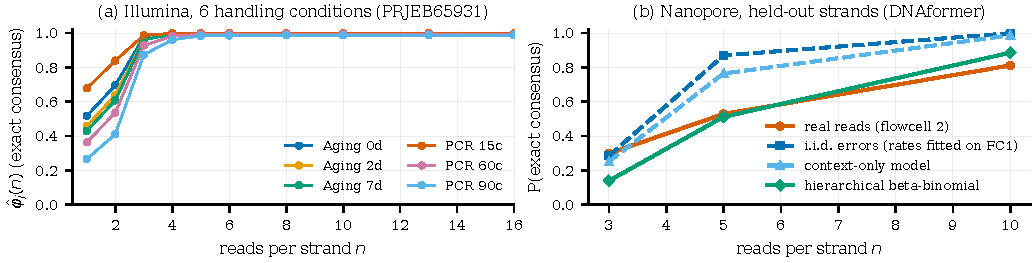
\includegraphics[width=\textwidth]{fig_consensus.pdf}
\caption{Real consensus-success curves.  (a) Six Illumina containers holding the same Twist pool
after different handling.  (b) Nanopore: real held-out strands versus error models fitted on
the other flowcell.}
\label{fig:consensus}
\end{figure*}

\subsection{Adaptive retrieval reduces sequencing cost (RQ4)}
Fig.~\ref{fig:cost} and Table~\ref{tab:baselines} compare policies on real recovery-time
matrices.  On the Twist pool the controller needs 6{,}902--9{,}114 fewer reads than the
oracle-tuned static plan (11--17\%; paired 95\% CIs exclude zero for every placement).  Because
the statistic involves a 0.99-quantile, the bootstrap intervals are asymmetric.  Combined with
placement, adaptive retrieval needs 44{,}753 reads against 67{,}938 for uniform placement with
fixed depth ($-34$\%).  On the independent Genscript pool, adaptive retrieval needs 577{,}653
reads against 650{,}709 for the oracle-tuned static plan ($-11$\%) and, with the best
container, 306{,}210 against 831{,}222 for uniform fixed depth ($-63$\%).  The pivotal score
\eqref{eq:score} and the coverage-greedy score are statistically indistinguishable in all
cases; the gain comes from hazard-based allocation and stopping, not from stripe-importance
weighting.  A heuristic static allocator that equalises expected coverage is
2.3$\times$ \emph{worse} than uniform on the Genscript pool because it over-reads the
near-dead container; the adaptive controller learns to avoid it.

\begin{figure*}[t]
\centering
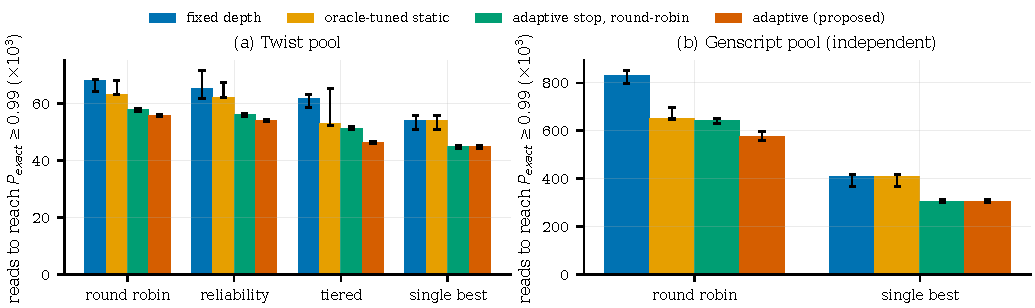
\includegraphics[width=\textwidth]{fig_cost_real.pdf}
\caption{Reads needed for exact recovery with probability $\ge0.99$ on real read streams
(200 read permutations for Twist and Genscript round-robin, 100 for Genscript single-best;
error bars: bootstrap 95\% CIs).}
\label{fig:cost}
\end{figure*}
\begin{table*}[!t]
\centering
\caption{Expected reads to reach exact recovery with probability $\ge0.99$ on replayed real read streams
(thousands; bootstrap 95\% CI in Fig.~\ref{fig:cost}).  Static plans pay their budget on every retrieval, so their
expected spend equals their 0.99-quantile; for adaptive policies the 0.99-quantile (``q99'', the budget a user must
provision) is shown separately.  $\Delta$: adaptive (pivotal) minus oracle-tuned static, paired over the same read
permutations (95\% CI).  With a single container, allocation is trivial and the gain is due to stopping only.}
\label{tab:baselines}
\footnotesize
\begin{tabular}{@{}llrrrrrrr@{}}
\toprule
Pool & Placement & Fixed & Oracle-tuned & Adaptive stop, & Adaptive, & Adaptive, & q99 of & $\Delta$ (95\% CI) \\
 & & depth & static & round-robin & cov.-greedy & pivotal & pivotal & \\
\midrule
Twist & round-robin (6) & 67.9 & 63.1 & 57.8 & 55.7 & 55.8 & 63.2 & $-7.3$ ($-12.1$, $-7.0$) \\
Twist & reliability-weighted & 65.4 & 61.9 & 56.0 & 54.2 & 54.1 & 61.8 & $-7.9$ ($-13.3$, $-7.6$) \\
Twist & tiered (4) & 61.9 & 53.1 & 51.3 & 46.4 & 46.2 & 53.0 & $-6.9$ ($-19.1$, $-6.2$) \\
Twist & single best & 53.9 & 53.9 & 44.8 & 44.8 & 44.8 & 54.0 & $-9.1$ ($-11.0$, $-6.7$) \\
Genscript & round-robin (6) & 810.4 & 617.9 & 639.9 & 532.1 & 531.9 & 694.2 & $-86.0$ ($-127.1$, $-78.8$) \\
Genscript & single best$^{\dagger}$ & 279.4 & 279.4 & 219.0 & 219.0 & 219.0 & 279.6 & $-60.4$ ($-70.5$, $-54.2$) \\
\bottomrule
\end{tabular}

\vspace{2pt}
\parbox{\textwidth}{\scriptsize 200 read permutations, except $^{\dagger}$100.  All policies completed in every trial.
The single-best container is chosen with the calibrated belief, which contains the evaluation-split leak of
Section~\ref{sec:eval}.  Superseded first-run Genscript numbers (computed before the per-strand consensus cache was
regenerated) are kept in \texttt{results/realdata\_genscript\_policies\_\{roundrobin,part2\}.csv}.}
\end{table*}


\subsection{Self-calibration from limited observations (RQ2)}
We replace the controller's belief by progressively less information: a generic literature
prior (yield 0.9, NB shape 10, dropout 0.5\%, a generic consensus curve; no reads of the pool),
beliefs whose coverage parameters are estimated from 1k--300k calibration reads per container
(binomial thinning of the calibration split, generic consensus curve), and full calibration
(300k reads plus per-run empirical $\hat\varphi_j$), each with prior sd $s\in\{0.5,1.0\}$
(100 read permutations, Twist round-robin).  All 14 configurations reach the target in every
trial and need 55{,}254--55{,}726 reads at 0.99 (Fig.~\ref{fig:limited}); the bootstrap CIs
overlap and the largest difference is 0.9\%.  With zero calibration reads the controller needs
55{,}584 reads (95\% CI 55{,}134--56{,}026), against 55{,}284 (54{,}800--55{,}778) with full
calibration, and both are well below the oracle-tuned static plan (63{,}142).  Online
calibration from the probe and the first batches therefore substitutes for an offline
calibration run \emph{on this pool}.  We caution that the Twist containers differ only
moderately (relative efficiencies 0.34--1.03), so the belief has little room to matter; the
harder test is transfer to the Genscript pool (RQ1, below).

\begin{figure}[t]
\centering
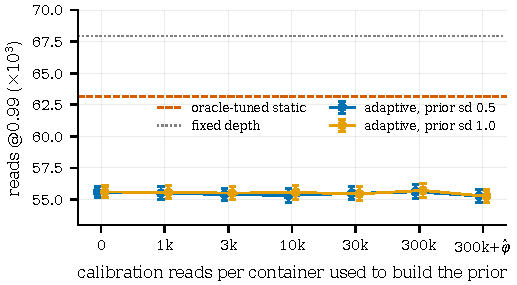
\includegraphics[width=\columnwidth]{fig_limited_calibration.pdf}
\caption{Self-calibration from limited observations (real Twist streams, 100 permutations):
reads at 0.99 versus the calibration reads used to build the controller's prior
(0 = generic literature prior).  Reference lines: oracle-tuned static and fixed depth
(200 permutations).}
\label{fig:limited}
\end{figure}

\subsection{Calibration of the posterior predictive (confidence)}
We set the budget to the median adaptive cost on the real Twist streams (55{,}600 reads), so
that about half of the retrievals complete within it, and record $\hat P_{\mathrm{complete}}$
\eqref{eq:pcomplete} after 30, 50, 70 and 85\% of the budget (200 trials; beliefs from full
calibration or the generic prior).  The estimate is strongly \emph{under}-confident
(Fig.~\ref{fig:confidence}): its mean is 0.04--0.22 while 52\% (full calibration) and 60\%
(generic prior) of retrievals complete; the expected calibration error is 0.30--0.60 and the
Brier score (0.31--0.60) is worse than that of a constant forecast (0.24--0.25).  It does rank
retrievals late in the budget: the AUC for predicting completion rises from chance
(0.49--0.56 at 30--50\% of the budget, CIs include 0.5) to 0.70--0.71 at 85\% (95\% CI
0.63--0.77).  Thus the posterior predictive is usable for ranking but not as a probability; this
explains why the futility rule built on it abandoned recoverable retrievals.  We have not isolated the cause; candidate explanations (untested) are the
spread-evenly allocation assumed for the remaining budget, which is worse than the controller's
actual allocation, and the normal approximation in \eqref{eq:pcomplete}.

\begin{figure}[t]
\centering
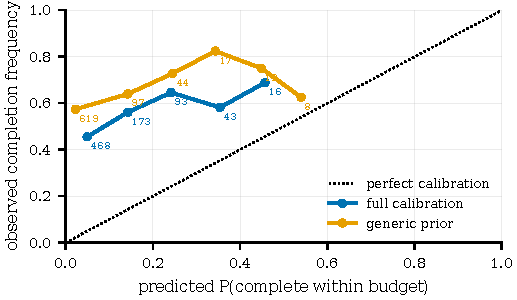
\includegraphics[width=\columnwidth]{fig_confidence.pdf}
\caption{Reliability diagram of the posterior predictive probability of completing within the
budget (real Twist streams, all checkpoints pooled; numbers: trials per bin; bins with fewer than 5 trials omitted).}
\label{fig:confidence}
\end{figure}

\subsection{Detecting changes in retrieval efficiency (RQ3)}
Table~\ref{tab:detect} evaluates the posterior at the read count where the prior model predicts
40\% recovery (``$R^\star$'', $\approx1$--2 reads per stored strand for most containers).  In
simulation (two containers degraded to relative efficiency 0.14) and on real streams (belief:
every container behaves like the fresh pool; the 90-cycle sample has relative efficiency 0.34),
the strongly degraded containers are flagged ($\Prob(\theta<0.7)>0.9$) in 100\% of trials, and
containers within 5\% of nominal efficiency are never flagged.  Posterior means track the true
relative efficiency on the real streams (0.28--0.29 vs.\ 0.34; 1.06 vs.\ 1.00--1.03) but
\emph{under}-estimate strongly degraded simulated containers (0.05--0.06 vs.\ 0.14).  Moderately
degraded containers are flagged occasionally: 2-day aging (0.76) in 10\% of trials at $R^\star$,
and 60 PCR cycles (0.75) in 73\% at $R^\star$ but 0\% at $2R^\star$.  However, nominal 90\% credible intervals cover the
true efficiency in only 0--83\% of trials: the binomial likelihood \eqref{eq:posterior} treats
strand recoveries as independent although coverage is correlated through $g_i$, so the
posterior is over-confident.

\textbf{Exploratory fix (overdispersed likelihood).}  Replacing the binomial in
\eqref{eq:posterior} by a beta-binomial with intra-container correlation $\rho_U$ (a
configuration option of the controller) widens the posterior.  We chose $\rho_U{=}0.01$ after
inspecting the Twist and simulated runs (selection set; 200 trials, same seeds, binomial
reference re-run in the same process): mean CI coverage rises from 0.08 to 1.00 on the real
Twist streams and from 0.51 to 0.79 in simulation, strongly degraded containers are still
flagged in 100\% of trials, the moderately degraded 60-cycle container is no longer flagged
(0.82$\to$0; the binomial re-run flags it in 82\% of trials versus 73\% in Table~\ref{tab:detect}, a run-to-run difference we have not fully traced; a candidate is process-dependent seeding, Section~\ref{sec:repro}), and mean absolute error of the posterior mean falls (0.060$\to$0.023 real,
0.038$\to$0.027 simulated); $\rho_U{=}0.05$ gives 100\% coverage everywhere, i.e.\ intervals
that are too wide.  On the \emph{held-out} Genscript pool with $\rho_U{=}0.01$ unchanged, mean
coverage over five containers rises from 0.01 to 0.85 (range 0.22--1.00), with no false flags
before or after; the near-dead PCR\_30c container (54\% dropout) is flagged in all trials under
both likelihoods (its relative efficiency, defined through finite recovery times, is not
meaningful and is excluded from coverage).  Posterior means on Genscript remain biased upwards
(mean absolute error 0.34) because the single multiplier $\theta_j$ cannot absorb the mismatch
between the fresh-pool belief and other containers' consensus curves.  This fix was not used in
any cost experiment above, and choosing $\rho_U$ from calibration data remains future work.
\begin{table}[!t]
\centering
\caption{Change detection at the prior-predicted 40\%-recovery point $R^\star$ (200 trials). Flag: $\Prob(\theta_j<0.7)>0.9$.
Cov.: coverage of the true value by the 90\% credible interval.}
\label{tab:detect}
\scriptsize
\setlength{\tabcolsep}{3pt}
\begin{tabular}{@{}llrrrrr@{}}
\toprule
Setting & Container & reads/strand & true eff. & post.\ mean & cov. & flag \\
\midrule
sim.\ s7 & C0 (degraded) & 1.17 & 0.14 & 0.06 & 0.02 & 1.00 \\
sim.\ s7 & C2 (degraded) & 1.66 & 0.14 & 0.05 & 0.00 & 1.00 \\
sim.\ s7 & C1 & 1.18 & 1.02 & 1.03 & 0.79 & 0.00 \\
sim.\ s7 & C5 & 2.20 & 0.96 & 1.02 & 0.83 & 0.00 \\
real Twist & Aging 0d & 1.08 & 1.00 & 1.06 & 0.05 & 0.00 \\
real Twist & Aging 2d & 1.08 & 0.76 & 0.81 & 0.37 & 0.10 \\
real Twist & Aging 7d & 1.08 & 0.90 & 0.82 & 0.03 & 0.00 \\
real Twist & PCR 15c & 1.08 & 1.03 & 1.06 & 0.00 & 0.00 \\
real Twist & PCR 60c & 1.08 & 0.75 & 0.63 & 0.31 & 0.73 \\
real Twist & PCR 90c (degraded) & 1.08 & 0.34 & 0.28 & 0.00 & 1.00 \\
\bottomrule
\end{tabular}
\end{table}


\subsection{Generalisation to an unfamiliar pool (RQ1)}
We run the controller on the Genscript pool---a different vendor, deletion-dominated errors,
coverage CV $\approx1.0$ and one near-dead container---with three beliefs: in-pool calibration,
a belief transferred from the Twist pool (mean Twist yield, NB shape, dropout and consensus
curve, identical for every container), and the generic literature prior (60 read permutations,
round-robin placement; static references recomputed on the same 60 matrices).
Table~\ref{tab:transfer} shows that every configuration completes in all trials.  Without any
in-pool calibration the controller needs 551.7--557.1k reads, 4--5\% more than with in-pool
calibration (528.9k; unpaired bootstrap CIs overlap), yet 10--11\% fewer than the
oracle-tuned static plan (621.0k) and 30--31\% fewer than fixed depth (798.2k).  The price of
an unfamiliar pool is paid mainly while the posterior learns which container is near-dead: it
sends 5.3--5.9\% of its reads there, against 3.4\% with in-pool calibration.  Prior width
($s=0.5$ vs.\ $1.0$) changes cost by less than 1\%.  Transfer across vendors thus costs a few percent rather than failing, but
on this harsher pool in-pool calibration still saves about 5\% (not statistically resolved with 60 trials).

\begin{table}[!t]
\centering
\caption{Generalisation to the unfamiliar Genscript pool (60 permutations; reads at 0.99,
thousands, bootstrap 95\% CI).  Share: fraction of reads sent to the near-dead container.}
\label{tab:transfer}
\scriptsize
\setlength{\tabcolsep}{3pt}
\begin{tabular}{@{}lrrr@{}}
\toprule
Policy / belief & $s$ & Reads (k) & Share \\
\midrule
Fixed depth (uniform, hindsight budget) & -- & 798.2 & 16.7\% \\
Oracle-tuned static (hindsight weights) & -- & 621.0 & -- \\
Adaptive, in-pool calibration & 0.5 & 528.9 (513.9--544.4) & 3.4\% \\
Adaptive, in-pool calibration & 1.0 & 529.0 (514.0--544.6) & 3.4\% \\
Adaptive, transferred from Twist & 0.5 & 557.1 (537.5--578.5) & 5.9\% \\
Adaptive, transferred from Twist & 1.0 & 555.8 (535.8--577.4) & 5.8\% \\
Adaptive, generic prior (0 reads) & 0.5 & 555.0 (536.3--574.6) & 5.5\% \\
Adaptive, generic prior (0 reads) & 1.0 & 551.7 (532.7--571.7) & 5.3\% \\
\bottomrule
\end{tabular}
\end{table}

\subsection{Exact recovery under container failures (RQ5)}
Removing one container's real read stream (Fig.~\ref{fig:failure}) shows how placement governs
degradation.  The single-container layout, cheapest without failures (44{,}473 reads), loses
the file when that container fails.  A four-container tiered layout (46{,}530 reads) remains
recoverable after any single loss, but losing one of its two main containers leaves few spare
fragments per stripe: retrievals then need 127--137k reads and complete within 3$\times$ budget
in only 45--48\% of permutations (losing a third container: 102k reads, always complete).  Round-robin
over six containers (55{,}610 reads) degrades by $+5$ to $+32$\% and always completes,
consistent with coupon-collector theory~\cite{barlev2025cover,levy2026expected}.
In simulation (12 retrievals per configuration, heavy errors), verification-gated stopping
produced no wrong output: with the default inner code (RS with four parity bytes, CRC-16) there
were 0 false fragment accepts in 10{,}567 decode attempts (95\% upper bound
$2.8\times10^{-4}$); with a deliberately weak code (two parity bytes, no CRC) 54--60 wrong
fragments per retrieval passed the inner check, all were caught by the stripe CRC or SHA-256,
and the retrievals ended \emph{partial} rather than wrong.

\begin{figure}[t]
\centering
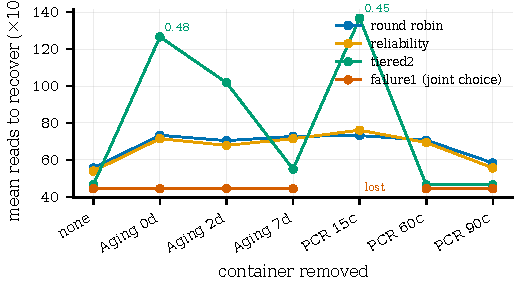
\includegraphics[width=\columnwidth]{fig_failure.pdf}
\caption{Real read streams with one container removed: mean reads of successful retrievals;
annotations give the completion probability within $3\times$ the 0.95-budget when below 1
(``lost'': unrecoverable).}
\label{fig:failure}
\end{figure}

\subsection{Ablation (simulated)}
Fig.~\ref{fig:ablation} removes one component at a time in a simulated scenario with correlated
failure domains (8 containers in 4 domains; 2{,}000 trials).  Removing adaptive allocation
(round-robin with adaptive stopping) costs $+79$\%; static reads cost $+68$\%; uniform or
independently optimised placement cost $+37$--$38$\% and lower reliability; ignoring correlated
failures in placement drops the success probability to 0.953.  Perfect channel knowledge
changes the cost by $<1$\% and coverage-greedy scoring is 1.5\% cheaper than pivotal scoring.
A seed sweep (five seeds) showed that the full design is the most reliable in 3/5 seeds but
does not reliably reach 0.99 in this scenario; we therefore do not claim that it does.

\begin{figure}[t]
\centering
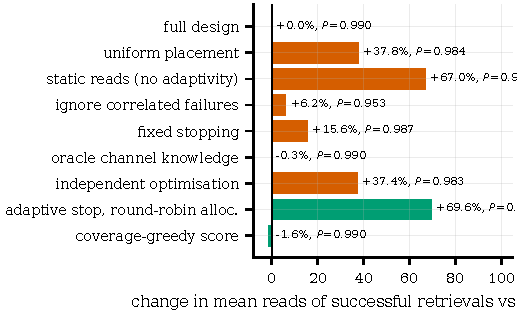
\includegraphics[width=\columnwidth]{fig_ablation.pdf}
\caption{Ablation in the simulated correlated-failure scenario (s4): change in mean reads of
successful retrievals and success probability $P$ (green: $P\ge0.99$).}
\label{fig:ablation}
\end{figure}

%=====================================================================
\section{Discussion}
%=====================================================================
\textbf{What drives the savings.}  Two mechanisms explain most of the gain: stopping as soon
as the data are provably decodable (the fixed plan must pay for the 0.99-tail on every
retrieval) and directing reads away from slow or dead containers once the posterior has seen a
few batches.  The second matters only when data are spread over several containers and their
efficiencies differ; it is irrelevant for a single container.  The more elaborate
stripe-importance weighting adds nothing measurable.

\textbf{Distribution is not free.}  When one container is reliable enough for the failure
budget, concentrating the data there is cheapest; spreading pays only if container loss must be
survived, and the post-failure margin $N-K$ minus the largest per-container load decides how
gracefully cost degrades.  The choice between these layouts is governed by the failure budget
$\varepsilon$, for which real per-container failure statistics do not yet exist.

\textbf{Model versus reality.}  Our analytical surrogate under-predicts real cost by 5--18\% on
the Twist pool and over-predicts it 3.7$\times$ on the Genscript pool.  Budgets derived from a
model should therefore be calibrated per pool; the self-calibrating controller is robust to
this because it uses the model only to rank containers and stops on verified decodability.

%=====================================================================
\section{Limitations and Threats to Validity}
%=====================================================================
Table~\ref{tab:limits} lists assumptions and limitations.  The most important are: (i) the six
``containers'' of each pool are aliquots of one synthesis batch sequenced on two flowcells, not
independently synthesised containers, and their coverage is correlated (69\% shared variance,
an upper bound for same-batch aliquots); (ii) container failures are injected, since no public
data report vial-level failure rates; (iii) recovery on real data is measured as exact
strand-level consensus against the design, a conservative proxy for inner decoding, because
our own encoding has not been synthesised; (iv) read costs are abstract and per-run setup
costs are zero, which favours many small adaptive batches (closer to streaming nanopore than
to Illumina flowcells); (v) the posterior is over-confident and the early-abandonment rule
based on \eqref{eq:pcomplete} abandoned 3.7--4.5\% of retrievals that would have succeeded, so
it is disabled.  Internal validity: all policies are compared on identical read permutations;
the fixed-depth and static baselines are given their best budgets in hindsight, which favours
them.  External validity: two Illumina pools from one study and two nanopore datasets.
\begin{table}[!t]
\centering
\caption{Assumptions, limitations and their consequence.}
\label{tab:limits}
\scriptsize
\begin{tabular}{@{}p{33mm}p{45mm}@{}}
\toprule
Limitation & Consequence \\
\midrule
Computational only (digital twin + replay) & no wet-lab confirmation; DT4DDS fidelity bounds external validity \\
DT4DDS default parameters, one archive geometry & conclusions may change with other codes, strand lengths, error regimes \\
Failures simulated (junk reads) & real failure modes and rates unknown; failure budget uncalibrated \\
Single efficiency multiplier $\theta_j$ & cannot represent dropout; adaptive allocators over-read near-dead containers \\
$\rho_U$ at the edge of its grid & selection coverage 0.87 $<$ 0.90; grid not extended post hoc \\
$\rho_U$ selected with $s{=}1$, runs use $s{=}0.5$ & selection and use not perfectly aligned \\
Calibration-optimal vs.\ cost-optimal $\rho_U$ differ & better-calibrated posterior made allocation costlier (post-hoc) \\
Gains in the mean only & no allocator, including the tail-aware one, lowers q99 \\
Replay is semi-empirical & oracle decodability; containers are aliquots of one batch \\
Abstract read costs, no setup cost & favours small batches; Illumina run economics not modelled \\
Reduced design for photolithographic scenario & 30 instead of 300 retrievals per policy \\
No theory (regret, optimality) & empirical claims only \\
\bottomrule
\end{tabular}
\end{table}


%=====================================================================
\section{Reproducibility and Availability}\label{sec:repro}
%=====================================================================
Code, tests, configuration, fixed random seeds, result files and the scripts that generate
every figure and table are in the project repository (Python $\ge3.11$; dependencies in
\texttt{requirements.txt}).  Public data are fetched by
\texttt{experiments/real\_data.py download} (ENA PRJEB65931; Zenodo 12666365, 17473983,
14296588).  An independent clean-environment reproduction (fresh clone and virtual
environment) passed all reproduction checks with byte-identical theory outputs.  Re-running an
experiment reproduces its numbers closely but not bit-for-bit: per-run
consensus-curve estimation is seeded through Python's process-randomised string hash, and we
observed small run-to-run differences (e.g.\ a flag rate of 73\% vs.\ 82\%) that we have not
fully traced.  Fixing this requires a stable seed derivation and a full re-run.  A claim-to-evidence
table mapping every reported number to its code and result file is provided with the
supplementary material (Table~\ref{tab:evidence} summarises it).
\begin{table*}[!t]
\centering
\caption{Claim-to-evidence summary (full table: \texttt{evidence/evidence\_traceability.csv}).  DT: DT4DDS digital
twin, full decode chain, no oracle.  Replay: real reads, oracle decodability.  No result is wet-lab evidence.}
\label{tab:evidence}
\scriptsize
\setlength{\tabcolsep}{3pt}
\begin{tabular}{@{}p{70mm}p{40mm}p{44mm}p{22mm}@{}}
\toprule
Claim & Command (\texttt{dt\_experiments.py} unless noted) & Result file (\texttt{results/}) & Evidence \\
\midrule
No wrong output, no false accept (Table~\ref{tab:safety}) & all DT runs & \texttt{dt\_*.csv} & DT \\
Verified stop: $-$27\% mean vs.\ best static reservation & \texttt{run}/\texttt{static baseline} & \texttt{dt\_baseline.csv}, \texttt{dt\_baseline\_static.csv} & DT \\
Model-based rules costlier than round-robin (baseline) & \texttt{run baseline} & \texttt{dt\_summary.csv} & DT, negative \\
Gains after outright failure (UCB $-$24\%); success set by redundancy & \texttt{run fail1}, \texttt{run fail2} & \texttt{dt\_fail\{1,2\}\{,\_static\}.csv} & DT, simulated failures \\
Crossover with severity of the worst container & \texttt{run sweep\_cov*} & \texttt{dt\_sweep\_cov*.csv} & DT \\
No rule lowers q99 & all DT runs & \texttt{dt\_summary.csv} & DT, negative \\
$\rho_U$ selection and held-out coverage & \texttt{calib}, \texttt{calib\_eval} & \texttt{dt\_calibration\_\{select,}\allowbreak\texttt{eval\}\_baseline.csv} & DT, partly negative \\
Forecasts over-confident, worse than climatology & \texttt{forecast baseline} & \texttt{dt\_forecast\_baseline.csv} & DT, negative \\
Binomial likelihood cheaper (post hoc) & \texttt{posthoc\_rho0} & \texttt{dt\_*\_posthoc\_rho0.csv} & DT, post hoc \\
Homogeneous control; photolithographic synthesis & \texttt{run homog}, \texttt{run photolitho} & \texttt{dt\_homog\{,\_static\}.csv}, \texttt{dt\_photolitho\{,\_static\}.csv} & DT (photolitho reduced) \\
Leak-free real-read replay & \texttt{paper\_experiments.py replay\_v3} & \texttt{replay\_v3\{,\_genscript\}.csv} & Replay \\
Leaky first analysis (upper bound only) & \texttt{real\_data.py policies} & \texttt{realdata\_*policies*\_v2.csv} & superseded \\
Correlated nanopore errors (MAE 0.083 vs.\ 0.181) & \texttt{q3\_correlated\_errors.py} & \texttt{q3\_summary.json} & real nanopore reads \\
Regret bounds; wet-lab containers; real failure rates & -- & -- & not attempted \\
\bottomrule
\end{tabular}
\end{table*}


%=====================================================================
\section{Conclusion and Future Work}
%=====================================================================
On real read streams from two independent pools, a self-calibrating controller that learns
container efficiency online, allocates reads by expected progress and stops on verified
decodability needs 11--17\% fewer reads for exact retrieval than a static plan tuned in
hindsight, and 34--63\% fewer when combined with placement; in simulation, verification-gated
stopping never produced a wrong file.  It works from a generic prior (cost unchanged on one
pool, $+$4--5\% on the other) and detects strongly degraded containers within one to two reads
per stored strand.  Its weaknesses are measured rather than assumed: over-confident efficiency
posteriors (largely corrected, in an exploratory held-out test, by an overdispersed
likelihood), an under-confident completion forecast, no benefit from stripe-importance
weighting, and a pool-dependent model bias.  The next steps are a wet-lab split-pool experiment
with independently synthesised, deliberately degraded and failed containers; choosing the
overdispersion from calibration data and recomputing the completion forecast by posterior
simulation; coupling the correlated-error model into the controller; and regret or optimality
guarantees for adaptive container selection.

\section*{Acknowledgment}
We thank the authors of the public datasets used here (ENA PRJEB65931, DT4DDS; DNAformer;
Srinivasavaradhan \emph{et al.}) for releasing reads together with designed sequences.

\bibliographystyle{IEEEtran}
\bibliography{references}

\end{document}
